
%Preambule

\documentclass {report}

% Import des extensions

\usepackage{hyperref}%pour insérer des liens
%\usepackage [francais]{minitoc}% permet de faire une table des matieres par chapitre
\usepackage  [francais,english]{babel} %il permet l'adaptation de LaTeX du français.
\usepackage [francais,nohints]{minitoc} % nohints permet d effacer l erreur des hints qu il y a quand on utilise les minitocs 
\setcounter{secnumdepth}{3}
%\setcounter{tocdepth}{2}
\setcounter{minitocdepth}{4}
\usepackage [T1]{fontenc} %il permet de spécifier à LaTeX l'utilisation du codage de caractères T1
\usepackage  [utf8]{inputenc} %gestion␣des␣accents␣
%\usepackage[latin1]{inputenc} %un package il permet d'utiliser les caractères ISO 8859-1

%\usepackage{listings} \lstset{ language=SQL, basicstyle=\small, numbers=left, numbersep=7pt, } %, numberstyle=\normalsize, 
%L'environnement  lstlisting L'environnement lstlisting permet de mettre en forme de façon colorée et d'utiliser de nombreuses options pour afficher du code.

\usepackage{verbatim} %L'environnement verbatim, accompagné du package du même nom, permet d'encadrer de gros volumes de code. Petit souci : il remplace les tabulations par des espaces.
%\usepackage{setspace}
\usepackage{parskip} % espace entre paragraphe
\usepackage{framed}
\usepackage{amssymb,amsmath,mathrsfs,mathtools}%package de math AMS et outils de math
\usepackage{color} % couleur
\usepackage{url}


%\usepackage[french]{minitoc}% permet de faire une table des matieres par chapitre
 %* Le package 'minitoc', disponible sur ftp://ftp.inria.fr/pub/TeX/CTAN/macros/latex/contrib/minitoc/, permet de construire une minitable des matières au début de chaque chapitre sous les classes 'book' et 'report'. Pour l'utiliser, il faut appeler les commandes \dominitoc avant la commande \tableofcontents habituelle. La commande \faketableofcontents permet de ne garder que les tables des matières locales et remplace alors la commande \tableofcontents. La commande \minitoc doit être appelée après chaque commande de début de chapitre \chapter dans lequel on veut inclure une table locale. A chaque appel de minitoc correspond un fichier .mtc<n> où n est le numéro du chapitre. Le compteur minitocdepth permet de fixer la profondeur des tables des matières désirées.

%\usepackage{lipsum}%Imprime du texte. Le paramètre optionnel permet de varier le texte imprimé.

\usepackage [pdftex]{graphicx} % gestion image
\usepackage [top=2cm,bottom=2cm,left=4cm,right=4cm] {geometry}%pour gérer les marges et dimension,la mise en page

%\usepackage{lastpage}%Il est possible de faire référence au nombre total de pages du document.  our obtenir un compteur de pages du type 1/3, 2/3, il faut charger dans le préambule du document le package lastpage.sty par la commande : usepackage{lastpage}Dans un champ de l’en-tête, il suffit alors d’insérer la commande :thepage/\pageref{LastPage}

%\usepackage[Sonny,Lenny]{fncychap} %Pour de beaux titres de chapitres dans vos documents, mettez dans le préambule \usepackage[Lenny]{fncychap} % Sonny, Lenny, Glenn, Conny, Rejne, Bjarne
%\usepackage{fancyhdr}%pour?les?en-têtes


% ajoute (entre autre) la bibliographie dans la table des matieres 
\usepackage[nottoc]{tocbibind}
\usepackage{natbib}
 
% biblio ordonnee classique
%\bibliographystyle{unsrt}
 

\usepackage{ragged2e} % justifie le texte

\hyphenation{intrusion}
\hyphenation{représente}
\hyphenation{automatique}
\hyphenation{exploration}
\hyphenation{construction}
\hyphenation{Utiliser}
\hyphenation{détection}
\hyphenation{outils}
\hyphenation{données}


%\usepackage{array}
%\usepackage{titlesec}%pour?les?sections
%\usepackage{titletoc}%pour?la?table?des?matières
%\usepackage{titling}%pour?le?

%\usepackage{hyperref}[pdftex]
%\usepackage[french]{varioref}

%\setcounter{secnumdepth}{1}
%\addto\captionsfrench{\renewcommand{\contentsname}{Sommaire}} %change le nom de la table de matieres

%fin 
%%%%%%%%%%%%%%%%%%%%%%%%%%%%%%%%%%%%%%%%%%%%%%%%%%%%%%%%%%%%%%%%%%%%%%%%%%%%%%%%%%%%%%




%%%%%%%%%%%%%%%%%%%%%%%%%%%%%%%%%%%%%%%%%%%%%%%%%%%%%%%%%%%%%%%%%%%%%%%%%%%%%%%%%%%%%%
%partie concernant la gestion des entêtes
%\pagestyle {fancy}
%\renewcommand\headrulewidth{2pt} %Ligne de séparation entre l'en-tête et le corps ,Pour forcer l’affichage d’une ligne horizontale, il suffit d’utiliser la commande \renewcommand{\headrulewidth}{1pt}, pour les en-têtes et \renewcommand{\footrulewidth}{1pt}, pour les pieds de page. détermine l'épaisseur du trait. Par défaut
%\renewcommand\headheight{2cm}

%\fancyhead[L]{\includegraphics [height=10mm,width=10mm] {ODM}} %haut de page gauche
%\fancyhead[R]{\includegraphics [height=10mm,width=10mm] {thumb-LOGO-UCAD}} %haut de page droite

%\fancyhead[C] {\leftmark}
%\fancyfoot[R]{\thepage/\pageref{LastPage}}

%\renewcommand\footrulewidth{2pt}%Ligne de séparation entre le corps et le pied de page,pour ne pas afficher de ligne horizontale, il suffit d’utiliser la commande \renewcommand{\headrulewidth}{0pt}, pour les en-têtes et \renewcommand{\footrulewidth}{0pt}, pour les pieds de page.
%\fancyfoot[C]{\thepage}
%\lfoot{Section \thesection}

%fin
%%%%%%%%%%%%%%%%%%%%%%%%%%%%%%%%%%%%%%%%%%%%%%%%%%%%%%%%%%%%%%%%%%%%%%%%%%%%%%%%%%%%%%




%%%%%%%%%%%%%%%%%%%%%%%%%%%%%%%%%%%%%%%%%%%%%%%%%%%%%%%%%%%%%%%%%%%%%%%%%%%%%%%%%%%%%%
%Redaction du document et enumerations des differentes parties 
%Corps du document
%Environnement

\begin{document}
% preparation des minitocs
\dominitoc
%\doparttoc

  %\dominitoc
	

\pagenumbering{roman} % numerote les page en chiffre romain 
% inclusion des chapitres
	
 %\include{Rett}
  

%%%% Réalisation de la page de garde

\begin{titlepage}
\begin{center}
%\flushleft
\includegraphics[height=30mm,width=30mm]{logo.jpg} %insérer un dessin
\hfill%
%\hspace*{10,5cm}
%\includegraphics[height=30mm,width=30mm]{logo_gbi.jpg}\\
%\begin{center}
%\centering
%\includegraphics[height=20mm,width=20mm]{institut_limerick.jpg}
%\hspace*{1cm}
%\flushright
\includegraphics[height=40mm,width=20mm]{logo_sfa.jpg}\\
\end{center}
\vspace*{1cm}



%%%%%%%%%%%%%%%%%%% Déclaration du type de document%%%%%%%%%%%%%%%%%%%%%%%%%
\begin{center}
\textsc{Universit\'e de Poitiers,}\paragraph{}
 Master 1 Réseaux de Télécommunications, Multimédia et Automatique
\end{center}


\begin{center}
\texttt{Rapport de projet de fin d'année\\
Du 05 Juin 2015} %textcolor c est pour mettre la couleur 
\end{center}
\vspace*{2cm}
 
 
\begin{center}
%\begin{framed}
% Commande permettant de définir l'écart
\setlength{\fboxsep}{2mm}
% Commande permettant de définir l'épaisseur du trait
\setlength{\fboxrule}{2mm}
\fbox{\textcolor{blue}{{{\textbf{\textit{\fontfamily{pnc}\selectfont{\huge{Outils algorithmiques pour la reconnaissance faciale.}}}}}}}}%textsc utiliser pour petite majuscule, \selectfont	active la police définie
%\end{framed}
\end{center}

%\vspace*{1.5cm}

%\begin {figure}[htbp]
 % \hbox{ 
 %    \includegraphics[scale=0.75]{intro}%[width=5cm]
 %    \hspace*{1cm}  %% pour mettre un espace (horizontal) de 5cm entre les deux images
   %  \includegraphics[scale=0.45]{intro1}
 % }
%\end {figure}

%\vspace*{1cm}

%\par \vspace{2cm}
%\begin{center}
%\includegraphics[height=60mm,width=60mm]{gaussienne.jpg}
%\end{center}
%\par \vspace{2cm}


  % emphasize mettre l'accent sur le texte mis en accolade
 %textbf pour mettre le texte en gras 


\begin{center}
\begin{tabular}{l r}

Groupe d'étudiants: &  \texttt{Ali \textsc{Toilha}}\\
& \texttt{Guy-Florent A. \textsc{Sadeler} }\\ % Partner names
&  \texttt{Viviane A. \textsc{Basse}}

\end{tabular}
\end{center}

\vspace*{1cm}
\begin{center}
\begin{tabular}{l r}
Responsable pédagogique: & \texttt{Pascal \textsc{Bourdon}}%\\
%& \texttt{David \textsc{Helbert}} % Instructor/supervisor
\end{tabular}
\end{center}

\end{titlepage}
	
	\newpage
	\null 
	\thispagestyle{empty}
	
	
	%\include{Rthanks}
	
	%\include{RabstractE}

	%\include{Rabstract}

	\tableofcontents %Insertion de lignes de pointillés avec dotfill

  %\setcounter{secnumdepth}{1}
	%\setcounter{tocdepth}{2} % On ajuste la profondeur


  %\selectlanguage {french}
	%\addcontentsline{toc}{chapter}{Table des Figures}
	%\listoffigures
	
	%\selectlanguage {french}
	%\addcontentsline{toc}{chapter}{Liste des Tableaux}
	%\listoftables

	%\include{Rquote}
	
	\pagenumbering{arabic}
	
	\chapter*{Introduction}
%\addcontentsline{toc}{chapter}{Introduction}
%\minitoc

At the University of Poitiers, students in Master (professional and research career) of Information and Communication Systems, Emphasis in Network Technologies field have to carry out a project during their first year in order to complete the training. This is the main reason we wrote this report of project.   
\paragraph{}
In fact, several topics were proposed to us and we choose the facial recognition for its multiplicity and variety in term of application fields, such as high security applications, remote monitoring and control of access etc. Indeed, this field is closely linked with human vision reproduction researche and the interaction between a machine and a human, which is a fascinating and booming subject.
\paragraph{}
Facial recognition consist in identifying a person with a picture of his face. It appears to be a quite active field in Vision from computer and Biomety. Recognition with an individual face is a skill of Biometry which is still to improve. Indeed, the acquired (captured) picture represents variation much higher than other characteristics (makeup, presence or absence of glasses, aging and expression of emotion). The method of face recognition is sensitive to the variation of the light and change the position of the face in the image acquisition. But still the system obtained is not yet able to adapt itself to certain kinds of variations on a face.
\paragraph{}
In fact, achieve the two prototypes necessary for our analysis we adopted the following outline anouncing this report. First, we define the project environment and aims at first, then we develop the state of the art methods to be programmed, as it were the theoretical concept. Then we establish a technical report is to explain the use of our prototypes made and finally we leave the analysis of the use of these prototypes to the comparison of our results.



	\chapter{Presentation of the project}
%\minitoc


\section{Context and scope of work}
\subsection{Context}
Previously carried out at the SIC Department of XLIM laboratory, the project we are in charge of implements "algorithmic tools and capturing software for facial recognition". This project interest was also interactions with and between users of a video game with an educational aim ("Serious game") by automatically animated avatars and experienced analysis difficulties, as well as the development of a software library for developers of video games on smartphones.
\paragraph{}
Facial recognition is often used as a tool to secure devices or control the use of applications. This technique both helps adults secure their systems and devices and parents limit and control access to systems for their kids.
The main idea was to improve parental control of tablets for children’s use. This could be helpful for parents wishing to use facial recognition to limit their children’s use past a certain time of a day.
\subsection{Scope of work}
This project aims to develop a facial capture software program (face recognition) in XLIM-SIC laboratory research work in collaboration with a company based in Lyon operating in the field of manufacturing tablets for children .
The required results at the end of this project are: facial recognition software program with
\begin{itemize}
\item Eigen Faces;
\item Fisher Faces.
\end{itemize}
Those will be programmed with multiple programming languages (Python, C ++).
This project is performed with the research professors of the Fundamental Faculty of  Sciences at the University of Poitiers: Pascal Bourdon and David HELBERT who  supervises the project


\clearpage


\section{Objectives }
The work required for this project is the development of a share recording software for the recognition of facial expressions for the identification of a face from an ID list in a home or for parental control.
Today innovation and the latest technologies are growing increasingly and allow the interactivity between human-machine to be maximal. Research  on facial expression is fundamental in many applications.
Facial recognition takes place in three stages, namely:
\begin{itemize}
\item Face detection
\item Extraction and normalization of facial features
\item Identification and / or verification
\end{itemize}
\paragraph{}
The main difficulty in face recognition is that  there are no two identical faces. Thus, each individual is unique and will be marked by gender, ethnicity, age or his haircut, but also by the shape, size and arrangement of the elements of the face.
\paragraph{}
This project has an educational goal because it contributes greatly to our engineering multimedia training, allowing us to put into practice the theories studied in the various teaching modules of our maste’sr degree (Image processing, tool and scientific computation, Algorithms for multimedia, random signal processing) but also by completing them. This project can be seen as a complement to our training.



\section{Deadlines}

 \begin{table}[!ht]%
\begin{center}
\begin{tabular}{|c|c|}
  \hline
  Deadlines & Deliverables  \\
  \hline
  \scriptsize{April 2} & Users requirements presentation + handouts \\
   \hline
  \scriptsize{May 13} & State of the art Theoretical \\
   \hline
  \scriptsize{June 11} & Official delivery (technical documents, codes, ...)\\
   \hline
  \scriptsize{June 18} & Project presentation\\
   \hline
   
\end{tabular}
\end{center}
\caption{\textbf{Deadline Table}}
\label{tab1}
\end{table}



	

	
	\chapter{State of the art}
%\minitoc


%%%%%%%%%%%%%%%%%%%%%%%%%%%%%%%%%%%%%%%%%%%%%%%%%%%%%
\section{Facial Recognition}
The challenge of face recognition can be formulated as followed :  with one or several images of a face, the goal would be to find or check the identity of a person by comparing his face to all the face images stored in a database. By the way this skill remains the most acceptable because it more suits with what human beings use in visual interaction; and compared to other methods, the face recognition seems more advantageous, in fact it is a non-intrusive method, in other words it does not require the cooperation of the subject, and a moreover the sensors used are cheaper.


\subsection{Facial recognition process}
Any facial recognition process must take into consideration several factors that contribute to the complexity of its task, because a face is a dynamic entity which constantly changes under the influence of several factors. A facial recognition system is generally  divided into the following steps (see the figure):

\begin{figure}[bth]%[!ht]
\begin{center}
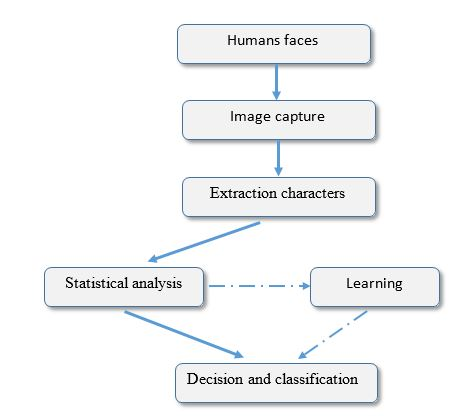
\includegraphics[scale=0.75]{fr_process}%[height=70mm,width=70mm]
\caption{\textbf{Facial recognition system process}}%
%\url {http://www.google.fr/}
\label{fr_process}%
\end {center}
\end{figure}

Facial recognition is facing the following problems:
\begin{itemize}
\item Change of pose ;
\item Light Variations ;
\item Variations of expression, age ;
\item Partial occultation of the face (concealing).
\end{itemize}

These variations are the most difficult because the variations in the appearance of a person face according to different pose or light conditions are often far more important than the variation between face images of two different individuals acquired under the same conditions.
This explains why pictures should be taken in specific conditions so that facial recognition can be efficient.

\subsection{The methods used for face recognition}	

Facial recognition methods can be classified into two broad categories: local and global methods. Amongst those methods, main ones will be presented thereafter.



\subsubsection{Global methods}

Global methods are based on well known techniques of statistical analysis. In these methods, face images (which can be shown as matrices of pixel values) are used as input of the recognition algorithm and are generally transformed into vectors, which are easier to handle. The main advantage of global methods is that they are relatively quick to set up in. However, they are very sensitive to variations of illumination, pose and facial expression.
\paragraph{}
The main existing methods are:
\begin{itemize}
\item The Principal Component Analysis (PCA) : EigenFaces
\item The LDA (Linear Discriminant Analysis) Algorithm : FisherFaces
\end{itemize}

\subsubsection{Local methods (Geometric)}

The local methods  include transformations applying to specific areas of the image, usually around characteristic points (corners of the eyes, mouth, nose, ...). Therefore, they require a priori knowledge on images. These methods are more difficult to implement but are more robust to the problems due to variations of illumination, pose and facial expression. The main existing methods are:
\begin{itemize}
\item EBGM (Elastic Bunch Graph Matching);
\item Modular Eigenface;
\item Hidden Markov Method.
\end{itemize}


But in fact, our aim on this project will be obviously to use both main global methods.

\paragraph{}

Both methods that we will present are using a common training algorithm steps that are :
\begin{itemize}
\item Preprocessing of training image set
\item Normalization and estimation of mean image
\item Use of PCA/ LDA
\end{itemize}

PCA/ LDA are statistical tools used to implement facial recognition method. For instance the use of PCA is divided into two steps :
\begin{itemize}
\item The determination of the input image weight from projecting input image into the face space and by multiplying the resulted vector to eigenfaces of the database.
\item A Comparison of results with metrics such as euclidian distance.
\end{itemize}


%%%%%%%%%%%%%%%%%%%%%%%%%%%%%%%%%%%%%%%%%%%%%%%%%%%%%
\section{Eigenfaces}
\subsection{Presentation of Eigenfaces}


	
The Eigenface approach began with a search for a low-dimensional representation of face images by Sirovich and Kirby in 1987.
It is the first method considered as a successful technique of face recognition. The Eigenface method uses Principal Component Analysis (PCA) to linearly project the image space to a low dimensional feature space and it is the name given to a set of eigenvectors when they are used in the computer vision problem of human face recognition

\subsection{Procedure}

A set of eigenfaces can be generated by performing a mathematical process called Principal Component Analysis (PCA) on a large set of images.
\paragraph{}
To create a set of eigenfaces, one must:
\begin{itemize}
\item Load a training set of face images. The pictures of  the training set should have been taken under the same lighting conditions, and must be normalized to line up the eyes ,mouths and other features.
\item Compute the average image : add each columns of the matrix T and dividing the previous obtained vector by the number of input images.
\item Subtract the mean from matrix T to obtain matrix S
\item Calculate the covariance matrix S.
\item Calculate the eigenvectors and eigenvalues of the covariance matrix S. Each eigenvector has the same dimensionality as the original images. The eigenvectors of the matrix  S are called eigenfaces.
\item Choose the principal components. The number of principal components k is determined arbitrarily by setting a threshold $\epsilon$ on the total variance.
\item Determinate the input image weight determination from projecting each image
\item Each image is represented by a vector which is used to reconstruct the images. We then save the average image, eigenfaces and the projection (weight ) of images.
\end{itemize}

This ends the training part of the implementation of eigenfaces and shows the skills used.



\subsection{EigenFaces flowchart}

The flowchart we  have to use is  divided into two basic parts: the learning phase and the identification phase where the Euclidean distance is used to calculate the difference between the weight of the image to be identified and the database images, then the program displays the nearest.
\paragraph{}
But retain before these two major steps,we have  pretreatments and it’s the phase which is carried out :
\begin{itemize}
\item The selection of the learning base ;
\item Reading images ;
\item The conversion of grayscale images ;
\item Resizing images ;
\item And finally the application of histogram equalization.
\end{itemize}


\begin{figure}[bth]%[!ht]
\begin{center}
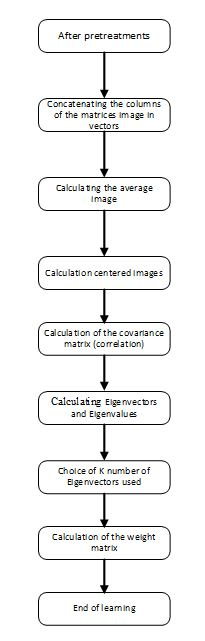
\includegraphics[scale=0.85]{ef_learningphase}%[height=70mm,width=70mm]
\caption{\textbf{EigenFaces flowchart learning phase}}%
%\url {http://www.google.fr/}
\label{ef_learningphase}%
\end {center}
\end{figure}	


\begin{figure}[bth]%[!ht]
\begin{center}
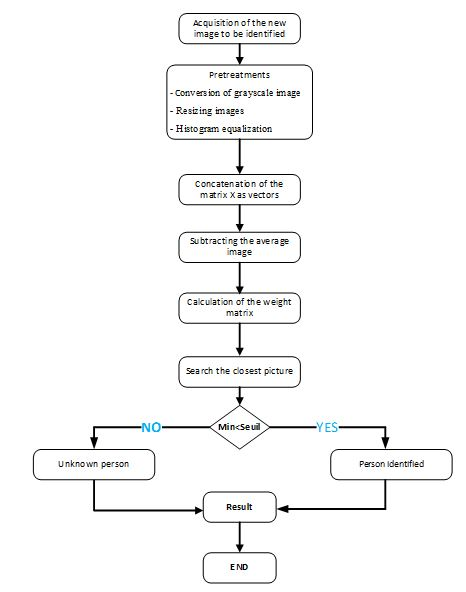
\includegraphics[scale=0.85]{ef_idphase}%[height=70mm,width=70mm]
\caption{\textbf{EigenFaces flowchart identification phase}}%
%\url {http://www.google.fr/}
\label{ef_idphase}%
\end {center}
\end{figure}	
 \newpage
\subsection{Benefits and deficiencies}	
\subsubsection{Benefits}	
Eigenface provides an easy and cheap way to realize face recognition in that:
\begin{itemize}
\item Its training process is completely automatic and easy to code. 
\item Eigenface reduces statistical complexity in face image representation.
\item Eigenface can used large databases.
\end{itemize}


\subsubsection{Deficiencies}
The deficiencies of the eigenface method are:
\begin{itemize}
\item Very sensitive to lighting, scale and translation;
\item Eigenface has difficulty capturing expression changes. 
\end{itemize}

The most significant eigenfaces are mainly about illumination encoding and don't provide useful information regarding the actual face.


%%%%%%%%%%%%%%%%%%%%%%%%%%%%%%%%%%%%%%%%%%%%%%%%%%%%%
\section{Fisherfaces}
Eigenface method uses PCA for dimensionality reduction, which yields projection directions that maximize the total scatter across all classes of images. This projection is best for reconstruction of images from a low dimensional basis. However, this method doesn’t make use of between-class scatter. The projection may not be optimal from discrimination for different classes.

While this is clearly a powerful way to represent data, it does not consider any classes and so a lot of discriminative information may be lost when throwing components away.

The Fisherface method is an enhancement of the Eigenface method that it uses Fisher’s Linear Discriminant Analysis (FLDA or LDA) for the dimensionality reduction. The LDA maximizes the ratio of between-class scatter to that of within-class scatter, therefore, it works better than PCA for purpose of discrimination. The Fisherface is especially useful when facial images have large variations in illumination and facial expression.

This projection maximizes the ratio of between-class scatter to that of within-class scatter. The idea is that it tries to “shape” the scatter in order to make it more reliable for classification.

\subsection{Linear Discriminant Analysis (LDA)}
The Linear Discriminant Analysis (LDA) is used to find the linear combination of characteristics that better separate  object or event classes. The resulting combinations can be used as a linear classifier, or generally in reducing characteristics before the posterior classification.

LDA is closely related to the PCA, because both seek the linear combinations of the variables that better represents the data. This statistic skill explicitly to model the difference between data classes unlike the PCA which does not take into account the differences between classes.
\subsection{LDA for recognition}
The LDA by recognition algorithm is divided into two phases, one for the calculation of person  models called system learning phase and the other which is to recognize a person thanks to registered models called test stage.
\subsubsection{Learning phase}
As in the PCA, it gathers the images of the learning database in a large image matrix T where each column represents a image listed Ti, then the average image is calculated.
For each class C, the average image is calculated.
Each image Ti of each class Ci is then refocused in comparison of the average. This produces a new image.
Then we proceed at calculation of the different scatter (dispersion) matrixes named as followed:
\begin{itemize}
 

\item The Intra-class Distribution Matrix;
\item The Inter-class Distribution Matrix;
\item Total Dispersion Matrix.
\end{itemize}
After we have defined the different dispersion matrixes, we must find the best projection that maximizes the intra-class dispersion on its matrix while minimizing inter-class dispersion, also on its matrix.

\clearpage
\begin{figure}[bth]%[!ht]
\begin{center}
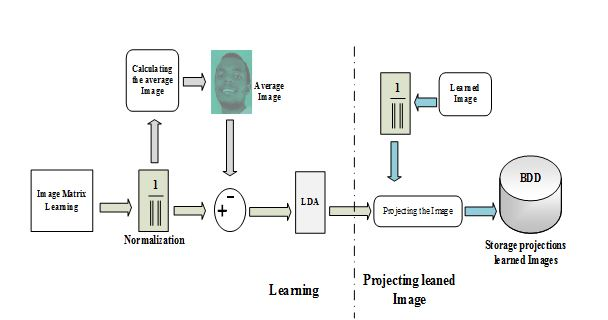
\includegraphics[scale=0.75]{learningPhaseGM}%[height=70mm,width=70mm]
\caption{\textbf{Learning phase of a face recognition system using a global method}}%
%\url {http://www.google.fr/}
\label{learningPhaseGM}%
\end {center}
\end{figure}
\subsubsection{Test phase or test stage}
Once the optimal projection that maximizes the found intraclass dispersion, the same pattern as the PCA on the projection of learned image and the projection of a test image is applied.
Then we project the test image in the Fisher space.
We compare the models obtained in learning phase. The comparison is made by calculating the distances (for instance, one can use calculation of the Euclidean Distance) between models and the test vectors and a decision rule is used to classify people.
\begin{figure}[bth]%[!ht]
\begin{center}
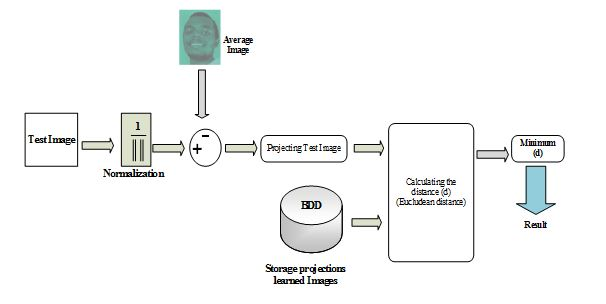
\includegraphics[scale=0.75]{TestphaseGM}%[height=70mm,width=70mm]
\caption{\textbf{Test phase of a face recognition system using a global method}}%
%\url {http://www.google.fr/}
\label{TestphaseGM}%
\end {center}
\end{figure}
\newpage
\subsection{Fisherfaces flowchart }
\begin{figure}[bth]%[!ht]
\begin{center}
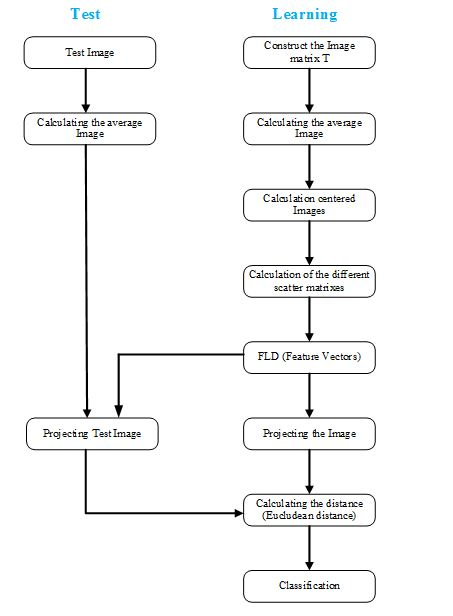
\includegraphics[scale=0.85]{test_learn}%[height=70mm,width=70mm]
\caption{\textbf{FisherFaces flowchart}}%
%\url {http://www.google.fr/}
\label{test_learn}%
\end {center}
\end{figure}

\subsection{Benefits and deficiencies}
The use of the LDA method for face recognition afford the following advantages:
\begin{itemize}
\item Maximizing inter-class scatter ;
\item Reduction of intra-class scatter ;
\item The method of Fisherfaces solves the problem of robustness to changes in pose, and facial expressions.
\end{itemize}

Despite these advantages, in the literature a serie of negative spikes still exists as:
\begin{itemize}
\item Costly (heavy) in computation time ;
\item Costly (heavy)  in memory space ;
\item Makes poor results when the number of training images is great.
\end{itemize} 


















 
 
 














































 
 
 
 
 
 
 
 
 




	\chapter{Organization}


\section{Project Management System}
In order to achieve our project on schedule we had to define steps to optimize the management of our time and to avoid delay on deadline.
%\paragraph{Step 1}
During early months at the launch of project, we started by writing the user requirements, which is a document etablished according to the need of the product owner. The user requirements allowing all users to orient the project progress and to keep in view the expected objectives. So this is a writing task. This  user requirements was presented to the product owner and before an academic jury.
This was about getting validation on user requirements of the product owner so that we make sure that his needs are clearly understood by us.
\paragraph{}
Then we had, thanks to Mister Chatelier's training a project manangement system called scrum. This system was about detailling all the tasks there was to complete and specifically the sprints.
\\In this part, we will describe the organization of our work throughout the project and will  present  tools used to the  project management.
%\paragraph{Step 2}
\newpage
For the project management,we used the Backlog and the Trello.
\subsection{ Backlog}
Thanks to the training given by Mister Christian Chatellier, we define the implementation of the project management system.
\\This system includes the backlog writing which listseach individual task there is to complete during the project and affords us to define every sprints (knowing that a sprint represents a week of work).
\\In the backlog all tasks are classified by priority and if a task contained in the backlog does not contribuate to the project objectives ,we must remove it
\begin{figure}[bth]%[!ht]
\begin{center}
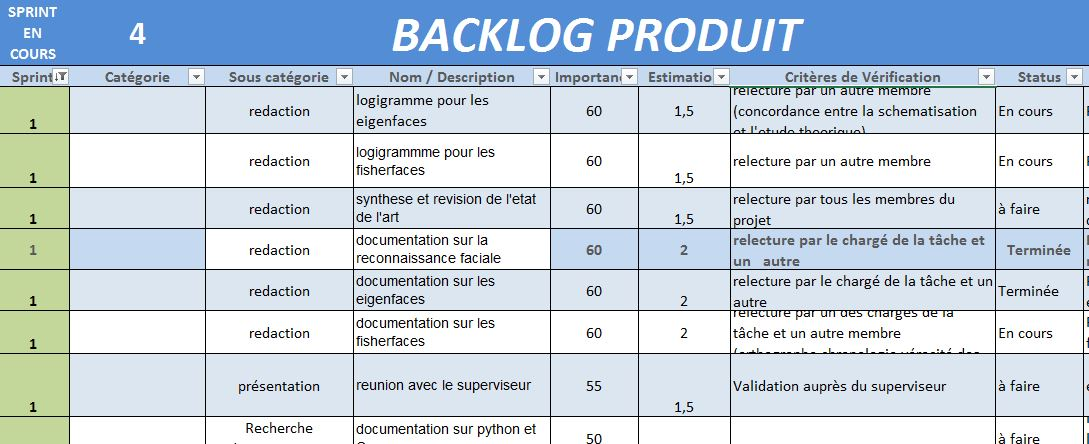
\includegraphics[scale=0.60]{baclog}%[height=70mm,width=70mm]
\caption{\textbf{Backlog}}%
%\url {http://www.google.fr/}
%\label{learningPhaseGM}
\end {center}
\end{figure}
\paragraph{}
In the backlog ,we have many parameters:
\begin{itemize}
\item Sprint:current sprint of a moment( a sprint correspond to a week)
\item Subcategory :  category of a task (redaction,research,programming or meeting with the product owner)
\item Name/description: description of a task
\item Importance : priority of task
\item estimation : time or duration for a task
\item criteria for verification
\item Status : indicates the status of a  task(doing,done)
\end{itemize}
Note that every friday we change the priority of certains tasks for praparing the next sprint.
\newpage
\subsection{Trello}
\subsubsection{Presentation}
The second tool used is Trello
Trello  is a project management tool allowing to list all project tasks.It is composed by many cards.
\\ With Trello we launch the scrum  every morning by a meeting between members of the group projet.It enables to see the progress work for all member  of the project.
\\our Trello is divides  into five cards:
\begin{itemize}
\item To do :list of all tasks that we have to do for  the week
\item Doing: list of current  tasks (Task  for a day)
\item Wait :tasks  waiting for very precise reasons
\item Test and Validation : task done but not yet tested
\item Done : Completed Tasks 
\end{itemize}
Note also that the project is divided into several weeks each corresponding to a Sprint.
\subsubsection{Sprint}
There we present the four sprint of the project :
\begin{itemize}
\item Sprint 1 
\\For this sprint we complete a second part which is the writing of the state of art. A document reporting the theoretical aspect to be developped in the project but also the explanation of the methods used and the algorithms to be programmed.During this sprint all intended tasks  have been completed
\begin{figure}[bth]%[!ht]
\begin{center}
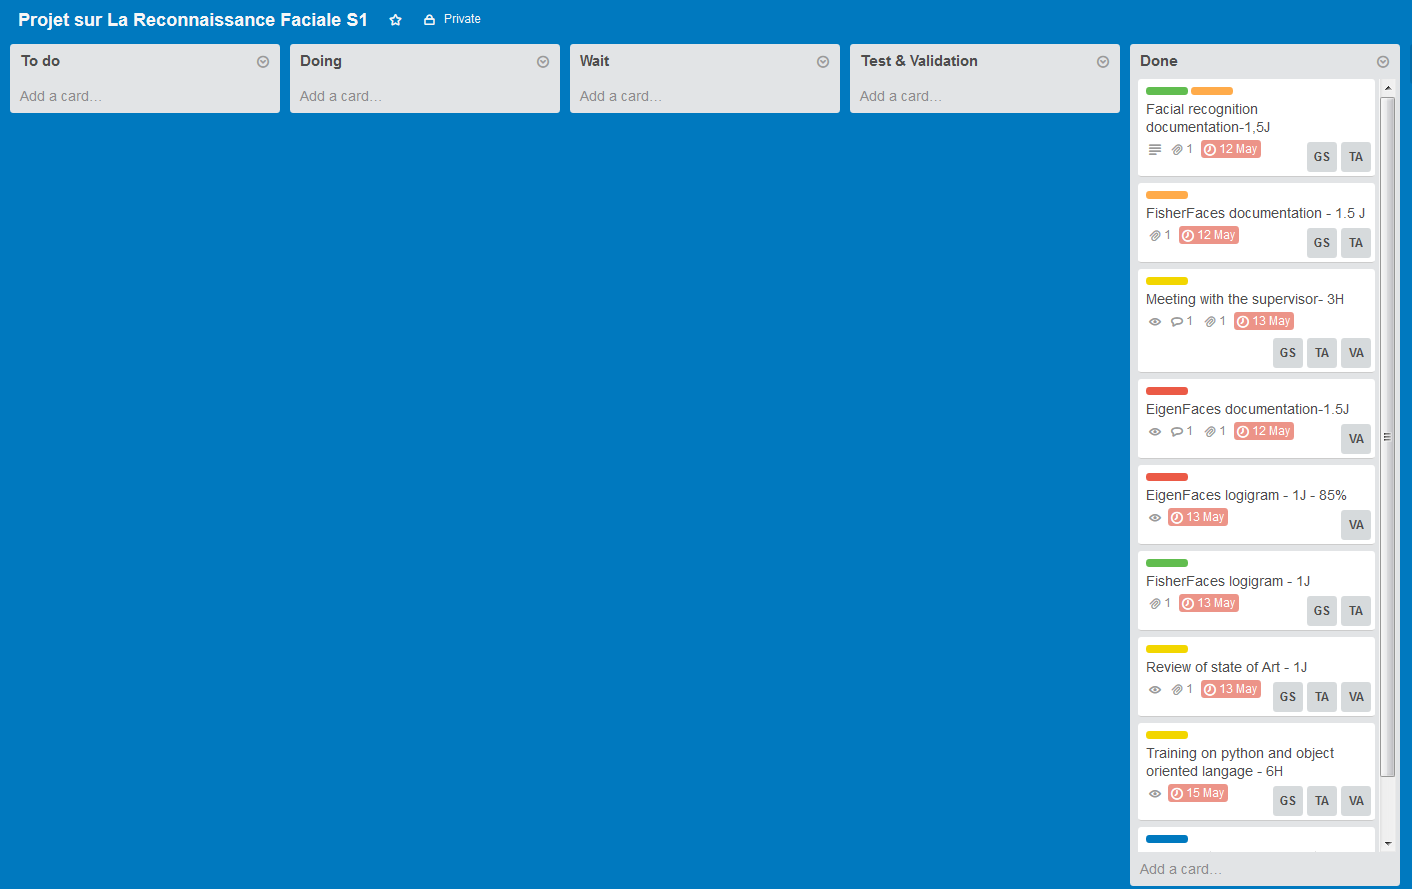
\includegraphics[scale=0.60,height=10cm,width=17cm]{sprint1}
\caption{\textbf{First sprint }}%
%\url {http://www.google.fr/}
%\label{learningPhaseGM}
\end {center}
\end{figure}
\newpage
\item Sprint 2 
\\At  the sprint 2, we did a literature search to deepen the appearance of algorithmic methods and presented the results of our research so that we all stand on the same point of view.We begin the prototype for eigenfaces method  in python. 
\begin{figure}[bth]%[!ht]
\begin{center}
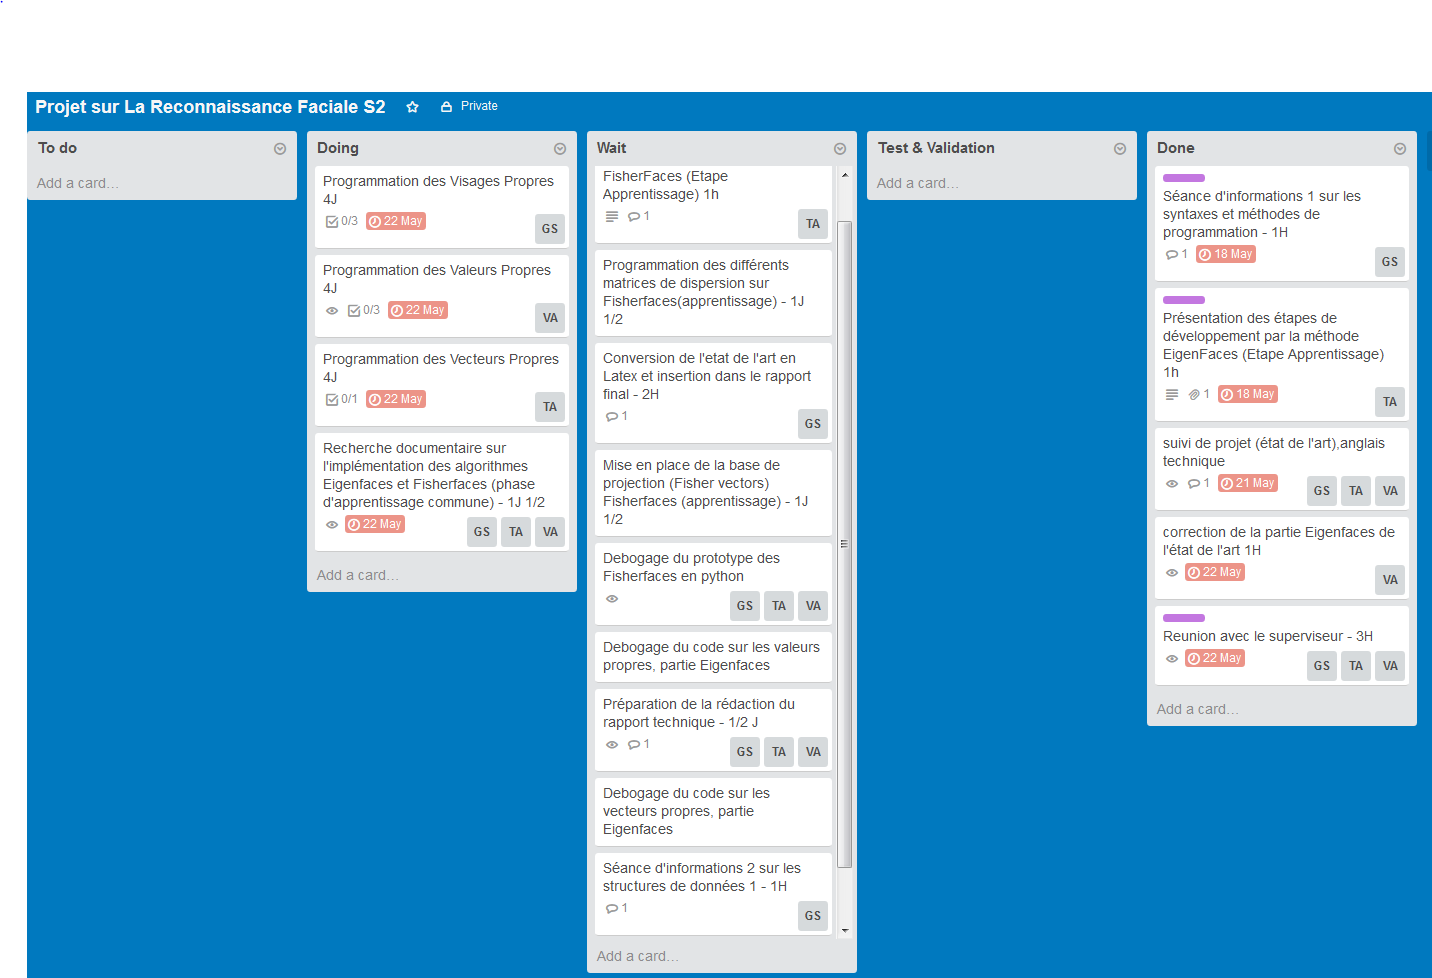
\includegraphics[scale=0.60,height=15cm,width=17cm]{sprint2}
\caption{\textbf{Second sprint }}%
%\url {http://www.google.fr/}
%\label{learningPhaseGM}
\end {center}
\end{figure}
\newpage
\item Sprint 3
\\This sprint consists in finishing the previous tasks started in later sprint about programming eigenfaces method. But added to those tasks we scheduled in the writing tasks. By the way some of the programming tasks  uncompleted  are renewed in Sprint 4.
\begin{figure}[bth]%[!ht]
\begin{center}
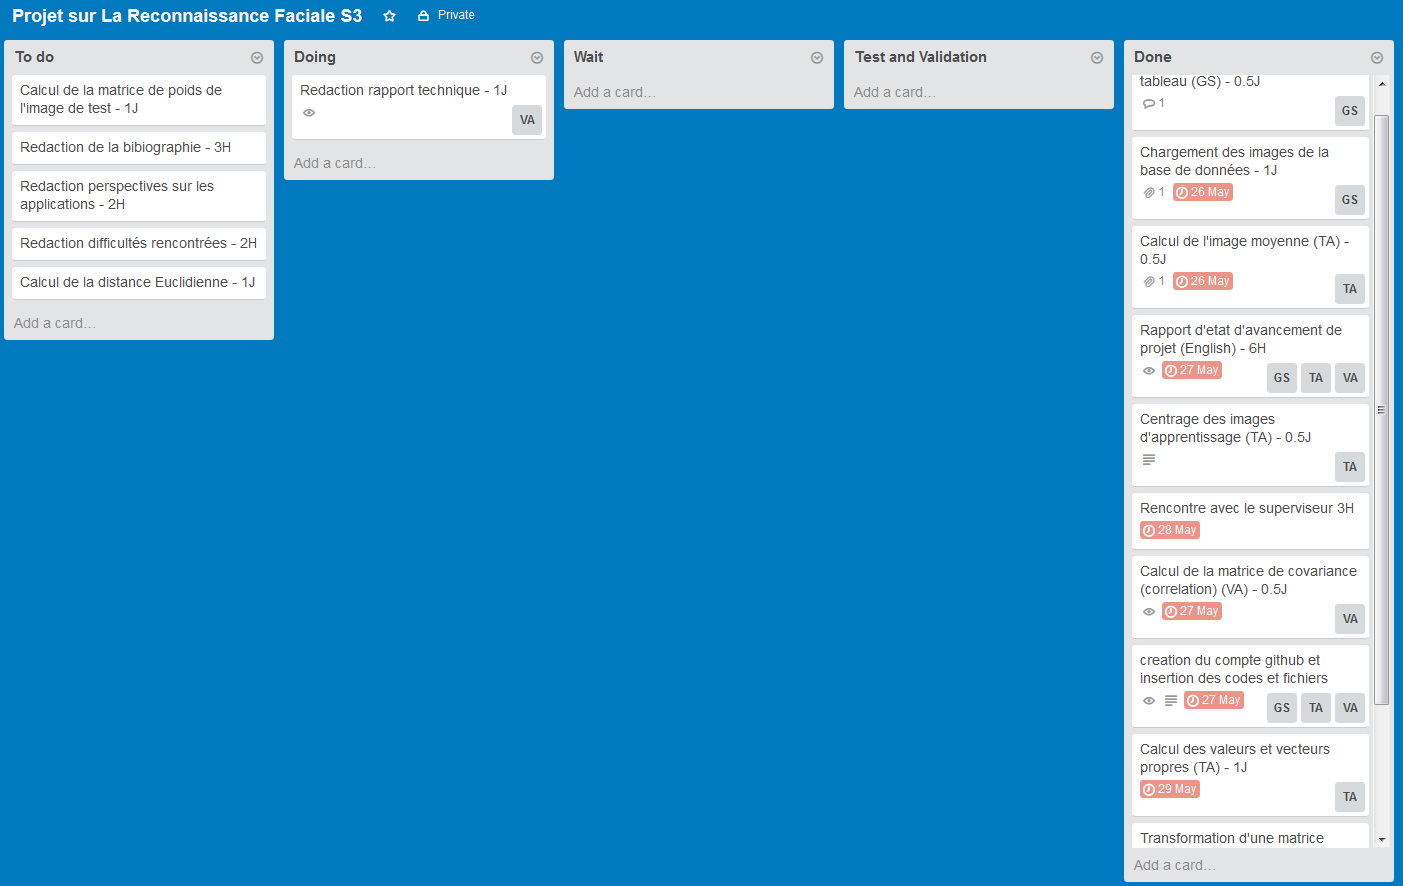
\includegraphics[scale=0.60,height=15cm,width=17cm]{sprint3}
\caption{\textbf{Third sprint }}%
%\url {http://www.google.fr/}
%\label{learningPhaseGM}
\end {center}
\end{figure} 
\newpage 
\item Sprint 4
\\For this sprint, we started by programming  Fisherfaces method but did not stop us to progress on the eigenfaces method.We also achieved some writting tasks.
\begin{figure}[bth]%[!ht]
\begin{center}
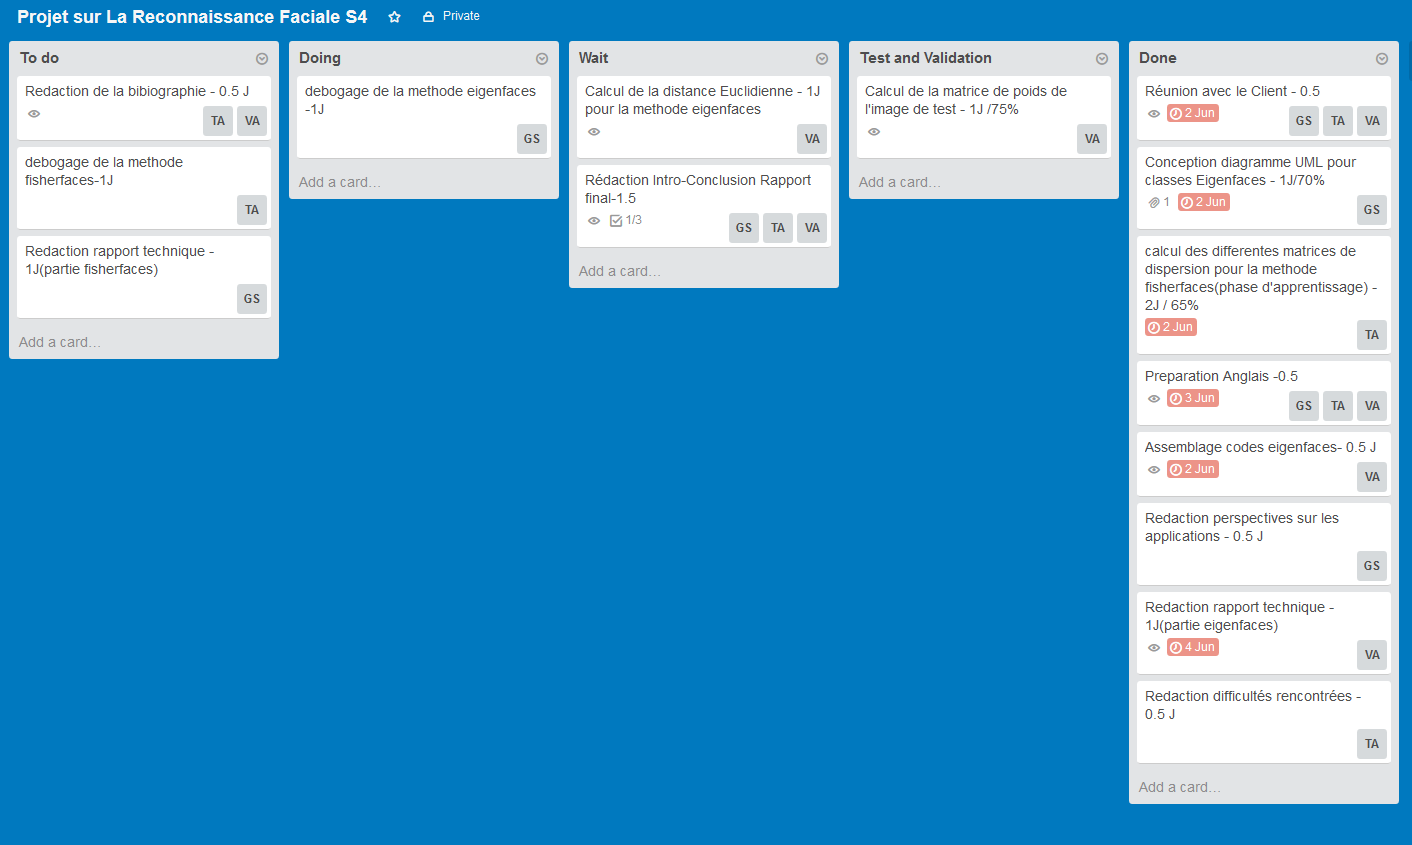
\includegraphics[scale=0.60,height=15cm,width=17cm]{sprint4}
\caption{\textbf{fourth sprint }}%
%\url {http://www.google.fr/}
%\label{learningPhaseGM}
\end {center}
\end{figure}


\end{itemize}

\clearpage
\section{Team Project}

The sponsor of this project is M. Pascal Bourdon working for XLIM-SIC Laboratory in Poitiers as a researcher. The results will be used by the Laboratory.
\paragraph{}
The project team includes :

Supervisors:
\begin{itemize}
\item	Pascal BOURDON as Supervisor and Product Owner;
\item	David HELBERT as Academic Training Principle;
\item	Christian CHATELLIER as Project Management Supervisor.
\end{itemize}
Students in charge:
\begin{itemize}
\item	Viviane Arame BASSE as Communication Manager
\item	Guy Florent A. SADELER as Technical Manager
\item	Ali TOILHA as Project Manager
\end{itemize}
The End users of this project are:
\begin{itemize}
\item	XLIM-SIC Laboratory,
\item	RTMA Training of the University of Poitiers for tutorials,
\item	Product owner and any potential company requiring facial recognition technology.
\end{itemize}
% Obvisoulsy, a Trello account was created from that document to allow us to hold a daily project meeting whiwh lasts fifteen minute and is called Scrum. Scrum is useful for daily monitoring of the current sprint.




%\paragraph{Step 3}
%Once, an organization detailling progressively every single task there is to complete and the different %actor on it we could more easily work on the programming part of our project to program the prototypes.
	\chapter{Technical report}
%\chapter{Application à la Transmission d’un fichier quelconque (*.mpeg, *.mp3, *.txt, *.doc, *.pdf, etc)}

%\minitoc


\section{Guide on Eigenface prototype}
In this section, we will explain the implementation of  eigenface  method  with the differents expressions used to program
\paragraph{}
Using mostly PCA (Principal Components Analysis), eigenfaces method is based on the calculation of eigenvectors and eigenvalues.
The algorithm consists of two steps:
 \begin{itemize}
 \item the learning phase : in which the protoype define a projection space with several person images; 
 \item and the identification phase  : which consist in projecting the face of the person one needs to recognize from the database.
\end{itemize} 
 Those steps are presented as followed :
\subsection{Learning phase}
 The learning phase can be divided into several steps:
 \begin{itemize}
 \item Step 1 : It is necessary to have an image database containing M images taken in good conditions. In our case we used the  \href{http://www.cl.cam.ac.uk/Research/DTG/attarchive:pub/data/att_faces.zip}{AT\&T picture database} contains 400 images. The database includes 40 subjects and each subject has 10 differents images of himself so that he can be easily recognised in differents conditions (with glasses, a hat, a smiling face for instance...). All these images are the basis for learning. Each image is a matrix.
 \item Step 2 :Each image matrix is converted into vector.










\parbox{0.60\linewidth}{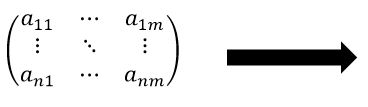
\includegraphics[scale=0.75]{matrice2vector}%[height=70mm,width=70mm]
}
\parbox{0.15\linewidth}{


%\begin{figure}[bth]%[!ht]
%\begin{center}
%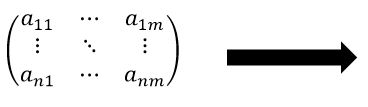
\includegraphics[scale=0.75]{matrice2vector}%[height=70mm,width=70mm]
%\caption{\textbf{conversion matrix to vector}}%
%%\url {http://www.google.fr/}
%\label{matrice2vector}%
%\end {center}
%\end{figure} 
\begin{displaymath} A=\left[\begin{array}{ccc}
a_{11} \\
\vdots \\
a_{nm} 
\end{array}\right] \end{displaymath}
}



\item Step 3 : Each image vector as previouly obtained becomes columns of a single matrix $\Gamma$. Every single image $\Gamma_{i}$ of the database is then in that single matrix and all of them are sorted from a subject to another. 
\begin{figure}[bth]%[!ht]
\begin{center}
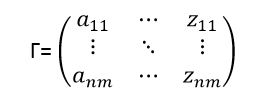
\includegraphics[scale=0.75]{grandematrice}%[height=70mm,width=70mm]
%\caption{\textbf{matrix of images database}}%
%\url {http://www.google.fr/}
\label{grandematrice}%
\end {center}
\end{figure} 
\\a:the subject 1 and z the subject n
\newpage
\item Step 4 : Calculate the average $\Psi$ of all images
\begin{figure}[bth]%[!ht]
\begin{center}
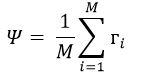
\includegraphics[scale=0.75]{moyenne}%[height=70mm,width=70mm]
%\caption{\textbf{average image}}%
%\url {http://www.google.fr/}
\label{moyenne}%
\end {center}
\end{figure} 
\item Step 5 : Substract the average image  from each image
\begin{figure}[bth]%[!ht]
\begin{center}
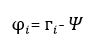
\includegraphics[scale=0.75]{centrage}%[height=70mm,width=70mm]
%\caption{\textbf{average image}}%
%\url {http://www.google.fr/}
\label{centrage}%
\end {center}
\end{figure}
\item Step 6 : Calculate the covariance matrix S
\begin{displaymath}
S= \sum_{i=1}^{M} \phi_{i} * \phi_{i} ^{T}= A * A ^{T} , A = (\phi_{1},\cdots \cdots  \cdots, \phi_{M})%\frac{1-q^{n+1}}{1-q}
\end{displaymath}

%\begin{figure}[bth]%[!ht]
%\begin{center}
%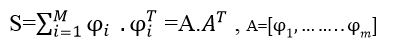
\includegraphics[scale=0.75]{cov_matrix}%[height=70mm,width=70mm]
%%\caption{\textbf{average image}}%
%%\url {http://www.google.fr/}
%\label{centrage}%
%\end {center}
%\end{figure}
\item Step 7 : After the covariance matrix ,eigenvalues and eigenvectors are computed.
Eigenvectors are then sorted by decreasing order.
%\begin{center}
%	\begin{tabular}{ll}
%	&\begin{math}
%		\sin \theta_{c} = n_{1}*\sin i_{c}\par \vspace{0.25cm}
%	\end{math}
%	\\

%{\color{red} \textbf{Formule de Snell-Descartes} :} & $n_{0}*\sin \theta_{c} = n_{1}*\sin i_{c}$ \\
%&  avec $n_{0} = 1$ (\emph{air})
%\end{tabular}
%\end{center}
\begin{center}
\begin{math}
   S * e_{i} =  \lambda_{i} * e_{i}
\end{math}


Formulas :
 $ \left\{\begin{array}{rl}
e_{i}= A * v_{i} & \mbox{eigenvectors } \\
\lambda_{i} = \mu_{i} & \mbox{eigenvalues
}\end{array}\right.$


\end{center}
  \end{itemize}
  
\subsection{Identification phase}  
The identification phase includes two steps and will help to recognize an input image in the image database.
 \begin{itemize}
 \item Step 1 : compute projection vectors
 
\begin{math}
   w_{k} = e^t_{k} * (\lambda_{i} -\psi)
\end{math} 
 
 
 

\paragraph{}
The projection vectors are called "weight vectors " and form a single matrix which will help for  compute  Euclidean distance. It also will help to find the class for an  input image.
\item Step 2 : compute the Euclidian distance
 
 \end {itemize}

This step in similar to the identification phase of Fisherfaces method.


 



%\begin{figure}[bth]%[!ht]
%\begin{center}
%\includegraphics[scale=0.75]{nom_image}%[height=70mm,width=70mm]
%\caption{\textbf{Titre image}}%
%\url {http://www.google.fr/}
%\label{label_image}%
%\end {center}
%\end{figure}

\clearpage
\section{Guide on Fisherfaces prototype}
This section is détailling differents steps on fisherfaces

\subsection{Learning phase}
The first part is also programmed into two steps the first step that is the learning phase is almost similar to fisherfaces' one. This similarity is onto the following common tasks:
\begin{itemize}
\item Loading of 10 images for every 40 subjects from the chosen database repertory;
\item Processing on images to get the mean image and center the images.

\end{itemize}

Once that common steps with eigenfaces are implemented or set up, we had to develop the LDA algorithm. This step can be describe as followed :
\paragraph{Calculation of the scatter matrices }
\begin{itemize}
\item Step 1 : We first get our $"y"$ list  gathering the numerotation of images according to the subject they belong to. Then this $"y"$ vector involved numbers from 0 to 39 since we have 40 subjects and each of this number are repeated ten times since every single subject has ten pictures. With the command $"c = np.unique(y)"$, we get the same vector in $"c"$ of numbers without them repeated tenth by sorting elements of $"y"$ and eliminating duplicates. Those numbers return the classes necessary to compute scatter matrix.
\item Step 2 : The second step will be to calculate the scatter matrices :

\begin{center}
	%\begin{tabular}{ll}
	 %&
		$Sw = Sw + np.dot((Xi-meanClass).T, (Xi-meanClass))$
		 Within classes scatter matrix (Sw)
	
	%{\color{red} \textbf{Within classes scatter matrix (Sw)} :}

\paragraph{}
%&  
$Sb = Sb + n * np.dot((meanClass - average).T, (meanClass - average))$
Between  classes scatter matrix (Sb)

%{\color{red} \textbf{Between  classes scatter matrix (Sb)} :} 
%\end{tabular}
\end{center}


\end{itemize} 
\paragraph{Calculation of fisherfaces }

\begin{itemize}
\item Step 3 :  We then apply the LDA algorithm to the previous reduced parameters
We need to find an optimal projection basis which both maximize the within dispersion relative to its matrix $Sw$ and minize the between dispersion relative to its matrix $Sb$.
\\
In other words, it consists in finding the "W" factor that maximize the Fisher optimizing Criteria :
%\begin{center}
%\begin{math}
%W= arg max_{T}(J(T))
%\end{math}
%\end{center}

\begin{center}
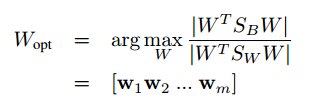
\includegraphics[scale=0.75]{critere_opt_fisher}%[critere_opt_fisher]
%\caption{\textbf{Titre image}}%
%\url {http://www.google.fr/}
%\label{label_image}%
\end {center}

\item Step 4 : We choose to use the PCA method to solve the problem we faced while trying to get W. The problem is about having matrices of different size. Then to resize them and be able to calculate W, PCA has been quite helful.



 
\end{itemize} 
\subsection{Identification phase}
The recognition of image from the basis obtained is similar to the previous method and take into consideration the calculation of distance such as euclidian distance, cosine \dots. We choose the euclidian distance.
	\chapter{Implementation}

\section{Configuration Management Guide}
In this section, we define a guide helping us programming and defining our structures in a homogene in order to easily read each other and to help the integration of our separate codes. This, since we programmed on the same prototype seperately. This document help us have homogenized codes on python.
\paragraph{}


\paragraph{Structure code :} For every languages used, we will prefer the definition of code in two parts:
\begin{itemize}
\item First part: definition of functions and procedures or methods;
\item Second part: Main function.
\end{itemize}


This process reduces the recall of certain calculations and allow to have a better visibility of code. It is necessary follow the order of definition for compilation.


\paragraph{Comments :} Each different parts should have a brief description before it is edited.
functions and procedures have a functional description;
tvariables are commented after their definition.


\paragraph{Definition of variables :} 
\begin{itemize}
\item Variables are defined at the beginning of each entity (functions, procedures, classes, hands etc ...) except possibly in object-oriented programming;
\item The name of a variable, whether local or global, is the simplest possible and defined in lowercase;


\item we will take care to separate input variables from those output for better visibility.
\end{itemize}

\paragraph{Definition of functions, procedures or methods :} 
\begin{itemize}
\item As with object-oriented programming (JAVA) we will take for a function, at least two significant words with the first word in lowercase letters and the first letter of the second word capitalized. It provides for example in case of two words "calculateMatrix" and three words "calculateScatterMatrix".
\end{itemize}


\paragraph{Definition of classes :} 
\begin{itemize}
\item Classes are defined in capital letters(first letter), they are the superior entities after the Object class.
\end{itemize}

\paragraph{Definition of Main :} 
\begin{itemize}
\item Before each function call comment out by a significant title.
\end{itemize} 

\paragraph{Identation :} 
\begin{itemize}
\item Carefully idente your code.
\end{itemize} 

\section{Implementation results}
As said lately,for the implementation of eigenfaces method we used AT\&T database  composed of 400 images. The database consists of 40 subjects and each subject has 10 images.

We illustrate hereinater some images of the database :
\begin{figure}[bth]%[!ht]
\begin{center}
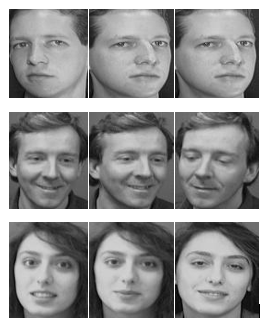
\includegraphics[scale=0.75,height=70mm,width=70mm]{capture_img}%[height=15cm,width=17cm]
\caption{\textbf{images of database }}%
%\url {http://www.google.fr/}
%\label{learningPhaseGM}
\end {center}
\end{figure}
\\All images of database are loading from directory by the function \textbf{read\_img.py}(annexes).
After that,the average of all images of the database will be calculated by the functiun \textbf{computeMeanImage\_.py} and centered by \textbf{computeCenteredImage\_.py}.
\\The average image is a vector and for saved it we needed to  convert it into a matrix(annexes).
\clearpage
The illustration of average image is :

\begin{figure}[bth]%[!ht]
\begin{center}
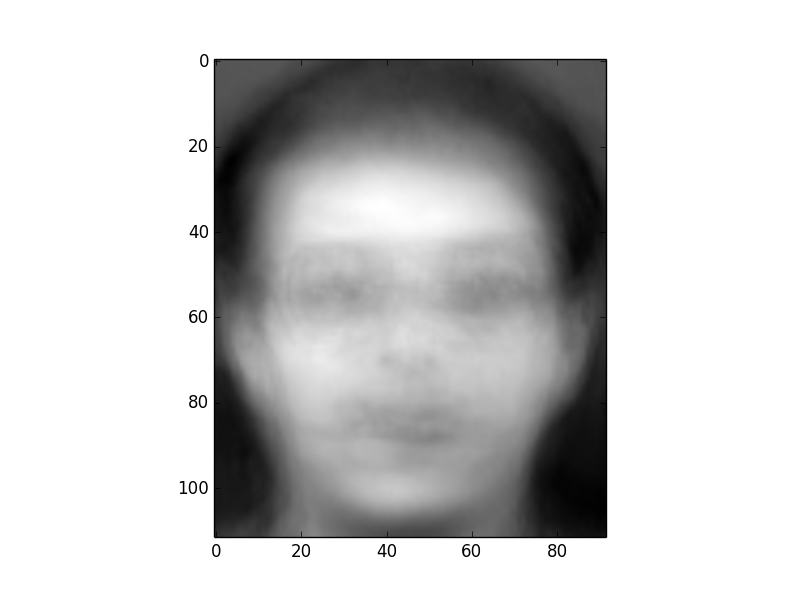
\includegraphics[scale=0.75]{figure_1}%[height=15cm,width=17cm]
\caption{\textbf{Average image }}%
%\url {http://www.google.fr/}
%\label{learningPhaseGM}
\end {center}
\end{figure}
The average image is fluzzy because many images are used.
\clearpage
\section{Integration into Oriented Programming Language}
In order to create Objects from our prototype we designed the main classes presented as following :

\begin{figure}[bth]%[!ht]
\begin{center}
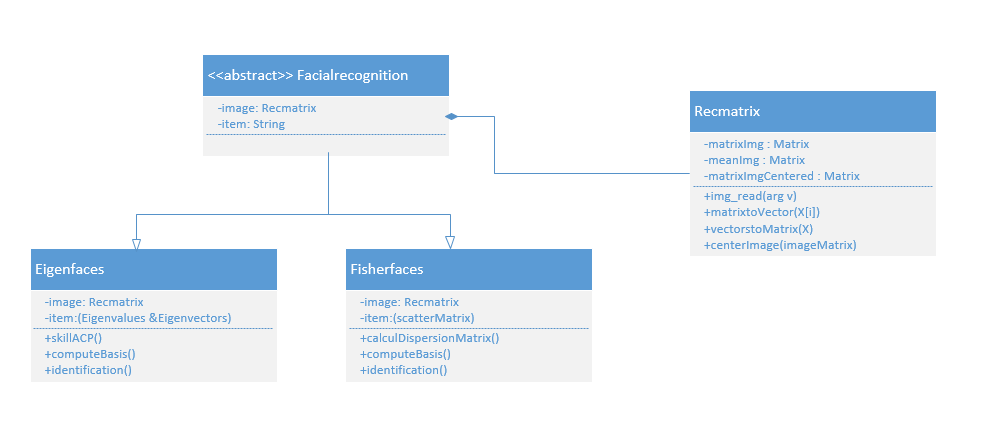
\includegraphics[scale=0.85,height=10cm,width=14cm]{diag_uml}%[height=15cm,width=17cm]
\caption{\textbf{UML Flowchart }}%
%\url {http://www.google.fr/}
%\label{learningPhaseGM}
\end {center}
\end{figure}


\section{Prospects}
Facial recognition develop tools very useful for people such as our first goals which were to improve parental control and to develop serious in order to help childrens with handicap. But so far, still there are some applications like high security, and ... All those applications require less human efforts, and then the use of this method are factor of unemployement and reduce responsibility from parents.
On this project, we would have expected to have much more time to implement the methods in other way and to optimize much more the programs.

\clearpage
\section{Difficulties faced and summary}
%\section{Difficultés rencontrés et Bilan}
\subsection{Difficulties faced}

When the project began, we set several objectives. To achieve them, we have established a  schedule for work organized. But throughout the project, we have encountered some difficulties: technical difficulties and organizational difficulties.
\paragraph{} 
The main difficulties are :
\begin{itemize}
\item implementation difficulties : because for programming methods, we had to define a unique way to structure the program for consistency in all codes. We have thus established a reference document to have uniform codes.
\item understanding difficulties :everyone had understood in a different way from others  the concept of the methods(eigenfaces and fisherfaces) for the implementation of our algorithm. 
\item Programming difficulties :we have different levels in programming. But that does not prevent us to program
\item Using tools  difficulties : everyone had to program a part of the code, so we needed a way for share and  synchronize our codes. the tool was new and we took time to control this,
\item management difficulties : as we have already said, we set goals and we had established a schedule for work in an organized way, but many secondary, unanticipated and unforeseeable tasks appeared.
\end{itemize}

However we faced all these difficulties, which allowed us to learn more about the two main domain of our project: images processing and programming language .
Finally, these difficulties may be helpful for future work. These can be apprehended in another project


\subsection{Summary}

This project allowed us to gain maturity in the work and help us  to understand the importance of schedule, organization, and discipline necessary to achieve a project. In addition, it also gave us the satisfaction of completing the project in a group. Each member benefits from the skills of other members. That share of skills and the adding skills we have gained make us think it is such a very positive experience to our training and future carreer. Because this experience has allowed us to figure out the complexity to manage a project, but also the difficulty of understanding and the importance of communication in a group.



	%\chapter*{Annexes}

Before creating functions,we imported different libraries.
\begin{figure}[bth]%[!ht]
\begin{center}
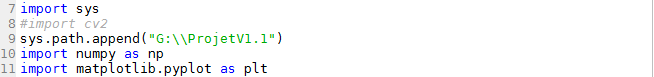
\includegraphics[scale=0.75]{import_bibliotheque}%[height=70mm,width=70mm]
%\caption{\textbf{jbbv}}%
%\url {http://www.google.fr/}
\label{read_}%
\end {center}
\end{figure}
\\The module sys gives direct acces to the arguments of the command line.
\\The module numpy is a digital library providing efficient support for large multidimensional arrays,and high-level mathematical funtiuns as linear algebra,statistics ...
\\The module Matplotlib is a library programming language that combined with python library numpy and scipy is a powerfull tool for tracing and visualizing data.
\section{Eigenfaces functions}
In this part ,we will put the different functions and their explenations
\begin{itemize}
\item Function used to load  images from directories
\begin{figure}[bth]%[!ht]
\begin{center}
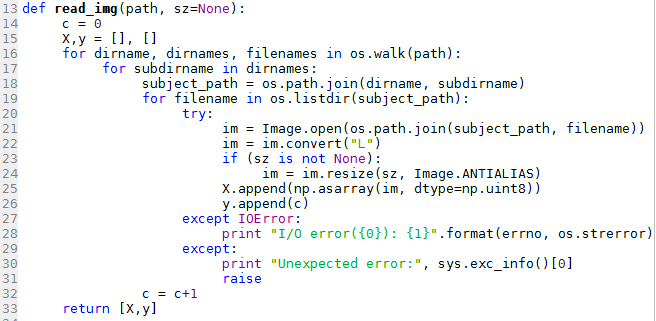
\includegraphics[scale=0.75]{fonc_ReadImg}%[height=70mm,width=70mm]
%\caption{\textbf{jbbv}}%
%\url {http://www.google.fr/}
\label{read_}%
\end {center}
\end{figure}
\\This function has input the full path to load all the images of the database.
It returns X which is a list of all the combined images and y which is the subscript i of all images for the subject i.
%\paragraph{}
\newpage
\paragraph{}
\item  Function used to transform matrix to vector
\begin{figure}[bth]%[!ht]
\begin{center}
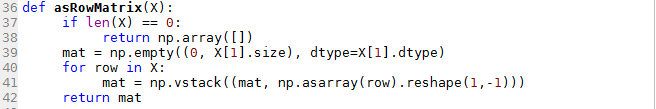
\includegraphics[scale=0.75]{fonc_marixVectors}%[height=70mm,width=70mm]
%\caption{\textbf{jbbv}}%
%\url {http://www.google.fr/}
\label{read_}%
\end {center}
\end{figure}
\\This function transforms an  images matrix  as a vector. It takes as input a matrix A and returns a vector mat.
\\The function vstack   returns  an vertical vector.
\paragraph{}
\item Function for calculating the average and centering all images
\begin{figure}[bth]%[!ht]
\begin{center}
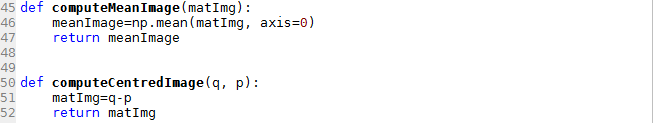
\includegraphics[scale=0.75]{fonc_mean_and_centred_img}%[height=70mm,width=70mm]
%\caption{\textbf{jbbv}}%
%\url {http://www.google.fr/}
\label{read_}%
\end {center}
\end{figure}
\\The function ComputeMeanImage takes as input the  matrix matImg and returns the average image for the  learning base.
\\ The function ComputeCentredImage center each image .The  average image is subtracted from each image
\\It returns back matIm:corresponding to the result of the image centered.
\item The function for calculating the covariance matrix
\begin{figure}[bth]%[!ht]
\begin{center}
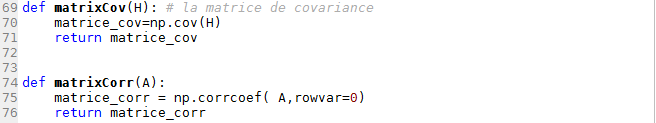
\includegraphics[scale=0.75]{fonc_matrix_cov_and_corr}%[height=70mm,width=70mm]
%\caption{\textbf{jbbv}}%
%\url {http://www.google.fr/}
\label{read_}%
\end {center}
\end{figure}
\\corrcoef  standardize the covariance matrix.
\newpage
\item Functions for calculating specific elements
\begin{figure}[bth]%[!ht]
\begin{center}
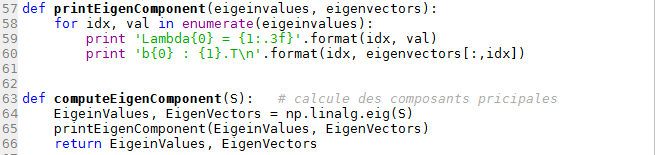
\includegraphics[scale=0.75]{fonc_print_and_compute_eigenvector_eigenvalue}%[height=70mm,width=70mm]
%\caption{\textbf{jbbv}}%
%\url {http://www.google.fr/}
%\label{read_}
\end {center}
\end{figure}
%\paragraph{}
\\The function printEigenComponent print eigenvalues and eigenvectors.
\\The function computeEigenComponent calculates  eigenvalues and eigenvectors. They are computed with the normalized covariance matrix.
\paragraph{}
\item Main funtion gathering invocation of other computing functions 
\begin{figure}[bth]%[!ht]
\begin{center}
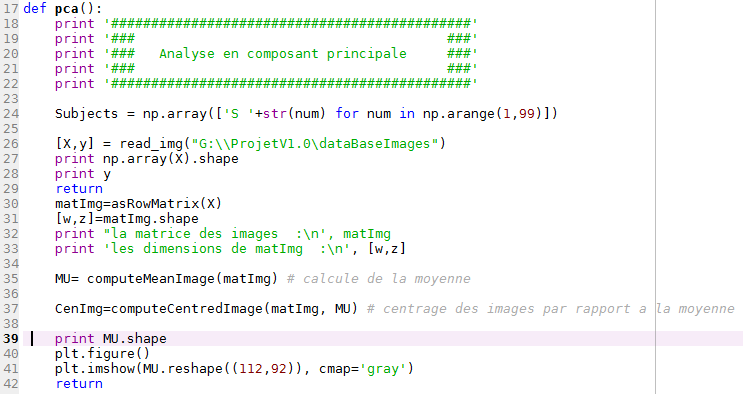
\includegraphics[scale=0.75]{affich_MeanImg}%[height=70mm,width=70mm]
%\caption{\textbf{jbbv}}%
%\url {http://www.google.fr/}
%\label{read_}
\end {center}
\end{figure}
\\This function allows to call others functions and create projection axes of eigenvectors and we also saved the average image.
%\clearpage
%\begin{figure}[bth]%[!ht]
%\begin{center}
%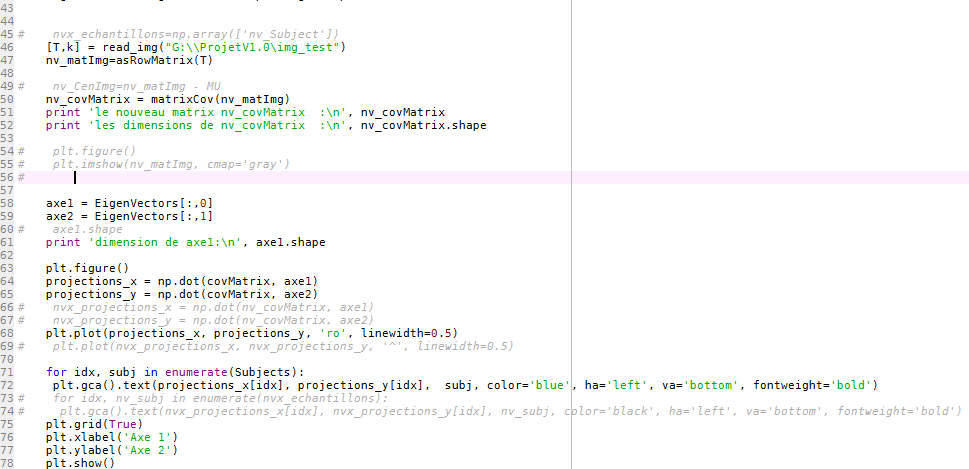
\includegraphics[scale=0.75]{fonction_pca1}%[height=70mm,width=70mm]
%\caption{\textbf{jbbv}}%
%\url {http://www.google.fr/}
%\label{read_}
%\end {center}
%\end{figure}
%\paragraph{}


\end{itemize}



	%\chapter*{Conclusion}
%\addcontentsline{toc}{chapter}{Conclusion}
%\minitoc

The objectif of the project was to develop a facial capture software program (face recognition) in XLIM-SIC laboratory research work in collaboration with a company based in Lyon operating in the field of manufacturing tablets for children.
\paragraph{}
To achieve this project, we used two methods to implement: the eigenfaces and Fisherfaces.
The eigenfaces using principal component analysis are a set of eigenvectors used in the field of vision to solve the problem of face recognition. The eigenfaces allow  to reconstruct a subspace retaining the best eigenvalues while keeping much useful information.
The Fisherfaces in turn use the LDA that analyze eigenvectors of the scatter matrix and aims to maximize the inter-class variations while minimizing the intra-class variations.
\paragraph{}
We have started with the implementation of  eigenfaces method in python. For that it was necessary for us to  have an image database. we used the ATT image database. However, some difficulties were encountered during programming which delayed us on objectives. That  why we focused on eigenfaces method and we could not make a comparison of the results of both methods


%\paragraph{}



	
 % \appendix

	
  %\include{Annexe}
	
 	\bibliographystyle{alpha} %classe les entrées par ordre alphabétique et les numérote en conséquence 

	\bibliography{biblio}
	
\end{document}

%Fin Redaction du document
%%%%%%%%%%%%%%%%%%%%%%%%%%%%%%%%%%%%%%%%%%%%%%%%%%%%%%%%%%%%%%%%%%%%%%%%%%%%%%%%%%%%%%